\documentclass[10pt]{article}
	
\usepackage[margin=1in]{geometry}		% For setting margins
\usepackage{amsmath}				% For Math
\usepackage{fancyhdr}				% For fancy header/footer
\usepackage{graphicx}				% For including figure/image
\usepackage{float}
\usepackage{hyperref}
\usepackage{tabto}
\usepackage{cancel}					% To use the slash to cancel out stuff in work
% avoid all eq numbering via:
\usepackage{mathtools}
\mathtoolsset{showonlyrefs}

\usepackage{cite}
\usepackage{url}
\usepackage{amssymb}                % To include mathbb symbols
\usepackage{graphicx}               % In preamble
\newcommand{\mcG}{\mathcal{G}}
\newcommand{\mcU}{\mathcal{U}}
\newcommand{\mcV}{\mathcal{V}}
\hypersetup{colorlinks=true,
            urlcolor=blue}
            
% Set up fancy header/footer
\pagestyle{fancy}
\fancyhead[LO,L]{Wearable Robotics 0360108}
\fancyhead[CO,C]{Final Project - Part 1}
\fancyhead[RO,R]{\today}
\fancyfoot[LO,L]{}
\fancyfoot[CO,C]{\thepage}
\fancyfoot[RO,R]{}
\renewcommand{\headrulewidth}{0.1pt}
\renewcommand{\footrulewidth}{0.1pt}
% \renewcommand{\thesubsection}{(\roman{subsection})}
\renewcommand{\thesubsubsection}{(\roman{subsubsection})}
\usepackage{algorithm}
\usepackage{algorithmic}


%%%%%%%%%%%%%%%%%%%%%%

\begin{document}
\begin{table}[h]
    \centering
    \begin{tabular}{l l l}
        \hline
        Name & ID & Email \\
        \hline
        Elad Siman Tov & - & elad.sim@campus.technion.ac.il \\
        \hline
        Eitan Gerber & - & eitangerber@campus.technion.ac.il \\
        \hline
    \end{tabular}
    \label{tab:personal_info}
\end{table}
\noindent Our code (.ino file) is \href{https://github.com/eladsimantov/Wearable-Robotics/blob/main/Final%20Project/Potentiometer_Servos.ino}{published on Github} for reference.
A video of the hand successfully opening and closing based on the potentiometer \href{https://technionmail-my.sharepoint.com/:v:/g/personal/eitangerber_campus_technion_ac_il/EebtvmOLvtBAnYd-IpQqAJ0BJ1s71PZn7ucrhZaetBrTBg?e=nfoBjf}{can be found here}.

% -------------------------------------- %
% --------- Assembly -------------- %
% -------------------------------------- %
\section*{Assembly}
We 3d printed and assembled a left hand according to the official guides.
During the assembly process we encountered some difficulties in understanding the instructions that were inconsistent and frequently skipped steps. We used the older version for the pulleys, which interfaces with the plastic connecting plate that comes with the servo motors as shown in figure \ref{fig:pulleys}.

\begin{figure}[H]
    \centering
    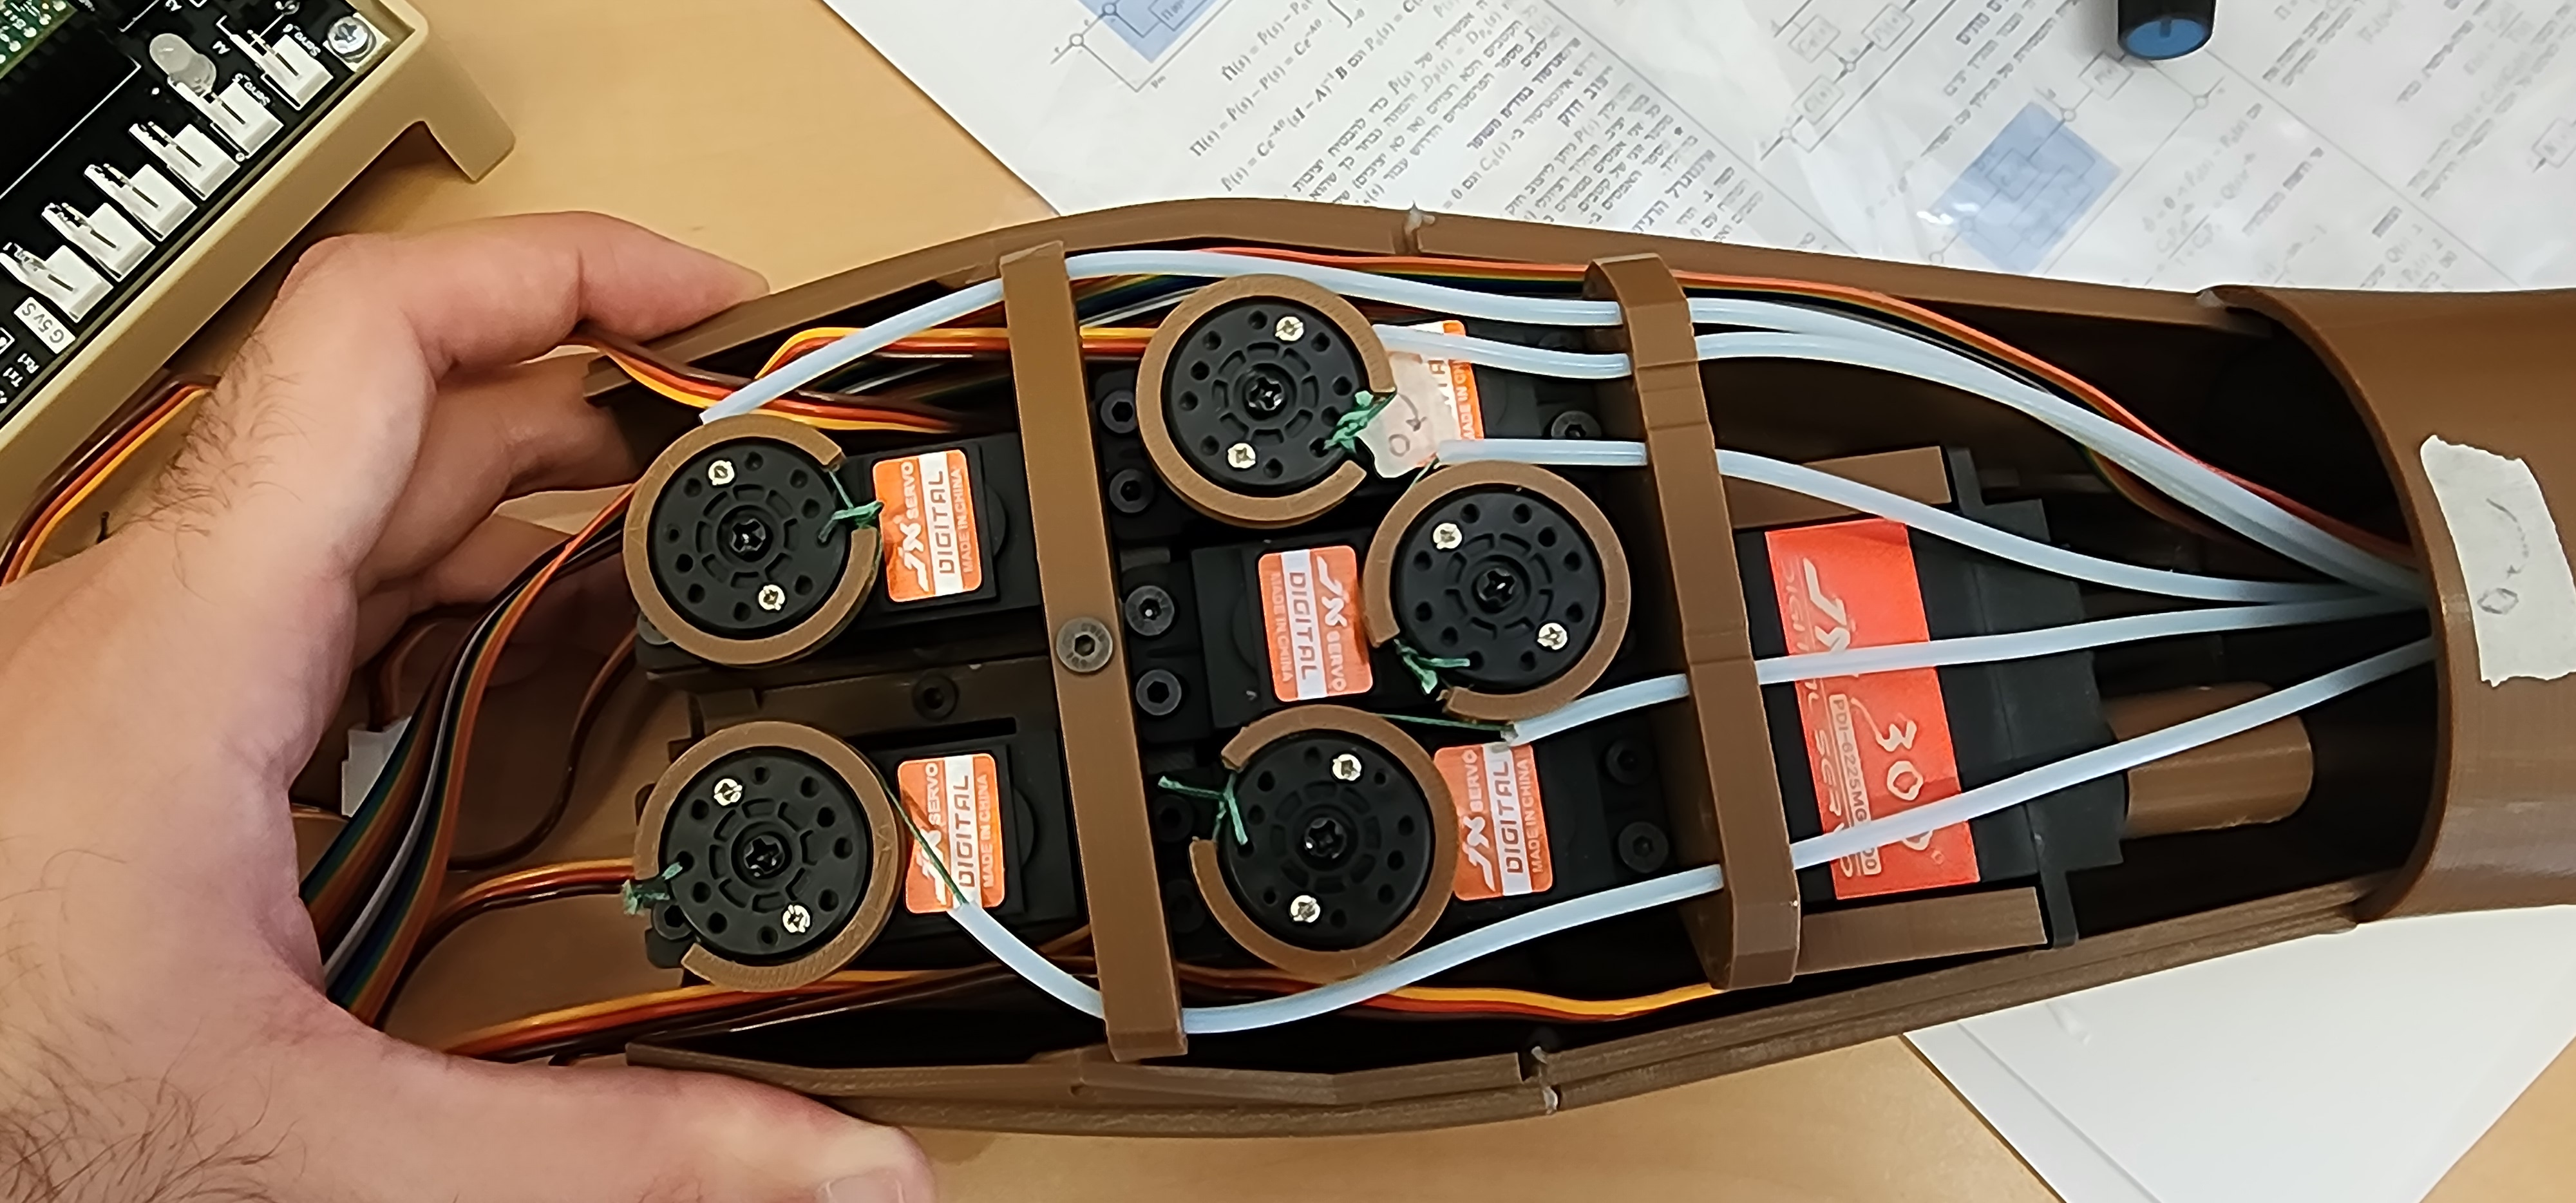
\includegraphics[width=0.5\linewidth]{Final Project/pulleys.jpg}
    \caption{The old version of the pulleys that were using in our robotic hand.}
    \label{fig:pulleys}
\end{figure}

\section*{Operation}
To demonstrate the operation of the hand we have programmed the micro-controller to map the potentiometer signal range (1024 bits) to the appropriate range of motion we have predefined for each servo motor corresponding to each finger or the wrist. 
The wrist servo motor was reset at its mid range position to allow for both supination and pronation actions. The rest of the servo motors (fingers) were reset to their zero position to avoid slacking the string driving each finger.
The video demonstrates the successful opening and closing of the hand before closing the cover of the hand to show the pulleys in action.

\end{document}